\section{循环结构}
在上一节,我们通过选择结构来实现一些``判断''的功能。但是我们的程序还有一些美中不足:它们只能单次运行。每次我打开这个程序,输入完毕再得到一次输出,然后程序就终止了。如果我想要多次输入,我就要反复打开程序——这就太麻烦了。所以我希望有一个程序,能够接收任意多次的输入,并在我给定某个条件后终止。循环结构就可以起到这样``反复执行''的作用。\par
\lstinline@for@ 循环和 \lstinline @while@ 循环都是常用的循环结构,而 \lstinline@do@-\lstinline@while@ 结构用得比较少。另有一些循环算法,比如 \lstinline@for_each@,我们留到精讲篇再介绍。\par
\subsection*{\lstinline@while@ 结构}
\lstinline@while@ 结构的基本格式是这样的:
\begin{lstlisting}
    while (<条件>) {
        <若干操作>;
    }
\end{lstlisting}
它与 \lstinline@if@ 结构非常相似,区别仅仅在于,\lstinline@if@ 结构中的内容只会运行一次;而 \lstinline@while@ 的内容可以反复运行(循环)。
\lstinline@while@ 结构的规则是:如果 \lstinline@<条件>@ 为真,那么执行 \lstinline@while@ 块内的若干操作;执行完毕后如果 \lstinline@<条件>@ 依然为真,那么再次执行若干操作。\par
那么我们就用 \lstinline@while@ 结构来修改一下我们的奇偶数判断程序,使它可以无限次接收输入——那意思就是需要无限循环。所以最简单的方法就是用 \lstinline@true@ 当作条件了,这样它就用远会执行下去。
\begin{lstlisting}
    int num; //定义num
    while (true) { //while的<条件>永远为true,所以它是无限循环
        cin >> num; //每次输入一个num的值
        const int mod {num % 2}; //num模除2的值
        if (mod == 1) { //如果mod为1满足,那么num就是奇数
            cout << "奇数" << endl;
        }
        else { //否则num就是偶数
            cout << "偶数" << endl;
        }
    }
\end{lstlisting}
这段代码的结构是 \lstinline@while@ 套上 \lstinline@if@-\lstinline@else@,有点像俄罗斯套娃。其实,这种结构与结构之间的\textbf{嵌套(Nesting)}在程序设计中是普遍存在的。\par
我们可以想像自己就是一个程序,按照顺序的方式执行代码,遇到 \lstinline@while@ 就检测要不要循环,遇到 \lstinline@if@ 就检测要走哪个分支,想必会更容易理解这种过程。\par
\begin{enumerate}
    \item 在程序定义了 \lstinline@num@ 之后,因为 \lstinline@while@ 的条件是 \lstinline@true@,所以循环块的代码开始执行。
    \item 当用户输入了一个值之后,程序会定义 \lstinline@mod@ 来存储 \lstinline@num@ 对 \lstinline@2@ 的模值。进下来判断 \lstinline@mod@,并给出相应的输出。至此,一次循环完成。
    \item 程序检测 \lstinline@while@ 的条件,因为条件是 \lstinline@true@,所以循环块的代码开始执行(回到上一步)。
\end{enumerate}
读者可以自行测试这个程序的功能。\par
让我们思考一下另一个问题:如果用户输入很多次之后要结束程序了呢?我们的 \lstinline@while(true)@ 结构就不尽如人意了——它永远不能自己停下来。虽然我们自己测试的时候可以用窗口上方的关闭按扭来强行关闭,但这一招并不是在任何时候都管用的。现在我们要想一种新的写法,用户可以通过输入特定的内容来结束程序。\par
一种思路是,输入 \lstinline@-1@ 结束程序。因为用户必须输入正整数,所以 \lstinline@-1@ 已经是非法输入了,不会与程序的正常功能相冲突。那么我们可以试着把这段代码写出来:
\begin{lstlisting}
    int num {0}; //定义num,这里必须初始化,因为while中就需要用到num的值
    while (num != -1) { //如果num不等于-1,就说明用户还需要继续输入
        cin >> num; //每次输入一个num的值
        const int mod {num % 2}; //num模除2的值
        if (mod == 1) { //如果mod为1满足,那么num就是奇数
            cout << "奇数" << endl;
        }
        else { //否则num就是偶数
            cout << "偶数" << endl;
        }
    }
\end{lstlisting}
这段代码看上去好像满足了我们的要求。但是真的是这样吗?以下是一个程序运行示例:\\\noindent\rule{\linewidth}{0.2pt}\texttt{
\textbf{5}\\
奇数\\
\textbf{8}\\
偶数\\
\textbf{1}\\
奇数\\
\textbf{-1}\\
偶数
}\\\noindent\rule{\linewidth}{0.2pt}
至此程序结束,但是好像出现了一些问题:
\begin{itemize}
    \item 输入 \lstinline@-1@ 之后,程序应该直接结束,而不是继续给输出一个结果,然后再结束。这说明我们的程序逻辑可能有一些问题。
    \item 另外,当我们输入 \lstinline@-1@ 之后,即便它多做了一次判断,也不该输出 ``\texttt{偶数}''这个结果。这说明我们的判断逻辑可能也有潜在问题。
\end{itemize}\par
我们先来分析第一个问题。其实只要你把自己想像成程序,然后模拟一下整个过程,就可以理解问题何在了。当用户输入 \lstinline@-1@ 之后,程序并不会直接终止,而是继续顺序执行``定义 \lstinline@mod@''``判断和输出''这些步骤。要解决这个问题,我们可以用后面讲到的 \lstinline@break@ 语句,或者把程序的逻辑修改成这样:
\begin{lstlisting}
    cin >> num; //在while块之外先接收一次输入
    while (num != -1) {
        //定义mod和选择结构部分的代码省略
        cin >> num; //在循环末尾接收下次输入,这样下一步就会进行条件判断
    }
\end{lstlisting}\par
另一个问题是我们的选择结构,貌似在输入 \lstinline@-1@ 时会判断为偶数。负整数并不是本程序的预期输出,所以这个问题可以无视;但出于知识学习的目的,我在这里需要讲一下。这个问题的根源在于我们的取余操作,\textbf{负数对正数取余得到的结果可能是负数}!\par
因此 \lstinline@-1%2@ 的结果是 \lstinline@-1@,它当然不等于 \lstinline@1@,所以就会被归入 \lstinline@else@ 状况之下,给出 \lstinline@"偶数"@ 的输出。\par
解决方法可以是把 \lstinline@if@ 的条件改为 \lstinline@mod==1||mod==-1@ ,用来判断负奇数;或者是直接用 \lstinline@mod==0@ 判断偶数,而把剩下的情况当作奇数来对待。以下是实现代码:
\begin{lstlisting}
    int num; //定义num,可不初始化
    cin >> num; //先输入第一个num
    while (num != -1) { //如果num不为-1,就继续循环
    	const int mod {num % 2}; //num模除2的值
    	if (mod == 0) { //判断是否为偶数
            cout << "偶数" << endl;
    	}
    	else { //mod可能是1或-1,我们把它们都归入else中
            cout << "奇数" << endl;
    	}
    	cin >> num; //接收下一个输出,下一步就会判断num是否为-1
    }
    cout << "程序结束"; //输出一个提示语,告诉用户程序结束
\end{lstlisting}
图3.9是这个程序的流程图,读者可以参考它来理顺这个代码的逻辑。\par
我们发现,这个程序不只可以判断正整数的奇偶,还可以判断负整数的奇偶。因此,它的功能可以得到拓展。不过这样就会出现一个新的问题——输入 \lstinline@-1@ 的时候怎么办呢?如果还把 \lstinline@-1@ 作为判断程序结束的标志,那我们就不能通过这个程序来判断 \lstinline@-1@ 的奇偶;如果输入 \lstinline@-1@ 的时候也要给出奇偶判断,那么我们就应该用新的方式来标记程序结束。比如说,如果用户输入一个 \lstinline@q@(或者别的字母),我们就结束程序。\par
\begin{figure}[htbp]
    \centering
    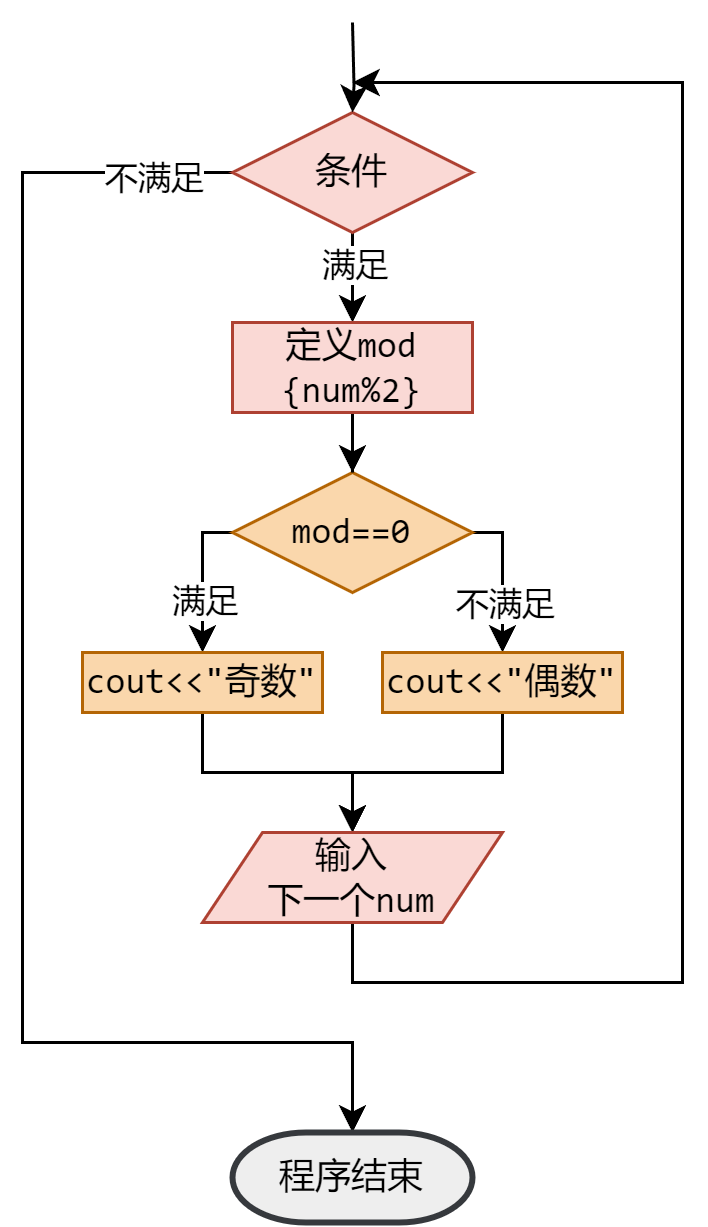
\includegraphics[width=0.6\textwidth]{../images/generalized_parts/03_structure_of_odd_or_even_with_while_loop.png}
    \caption{while循环奇偶判断流程图}
\end{figure}
这种实现方式是可行的,并且相当好用。我在这里先放代码,然后再做解释:
\lstinputlisting[caption=\texttt{while循环奇偶判断.cpp},label=lst:OddOrEvenWithWhileLoop]{../code_in_book/3.3/while循环奇偶判断.cpp}\par
这里最巧妙的操作在于使用 \lstinline@cin>>num@ 作为 \lstinline@while@ 循环的判断条件。前面我们提过,\lstinline@cin>>num@ 的返回值还是 \lstinline@cin@ 本身。而 \lstinline@ostream@ 类重载了 \lstinline@operator bool@,所以作为 \lstinline@ostream@ 类的对象,\lstinline@cin@ 可以被隐式类型转换为 \lstinline@bool@ 类型,这是它能作为判断条件的前提。\par
那么什么情况下 \lstinline@cin@ 会被隐式类型转换为 \lstinline@true@ 呢?就是在输入状态一切正常的情况下。在C++中,有很多情况会导致输入状态不正常,比如:
\begin{itemize}
    \item 期望输入的是一个整数,但输入了非数字的字符,或者输入了浮点数\footnote{输入浮点数的情况更加特殊,程序会把小数点之前的部分单独作为一个整数来处理(表征出来就是,多循环了一次),而将小数点作为非数字字符阻断,留到下次输入。}。
    \item 遇到了 \lstinline@EOF@\footnote{文件结尾(End-of-file)是一个特殊的标记,表示程序不能再从信息源读取更多信息。EOF不是ASCII中的一部分,不过有些系统会用值为 \lstinline@-1@ 的字符型数据来表示它。}。
    \item 其它可能导致I/O错误的软/硬件问题。
\end{itemize}
一般情况下 \lstinline@cin@ 的状态是正常的,转换为 \lstinline@bool@ 类型后返回 \lstinline@true@;而一旦遭遇这些情况,\lstinline@cin@ 的状态就会改变,从而转换为 \lstinline@bool@ 类型后返回 \lstinline@false@。\par
所以说,\lstinline@while(cin>>num)@ 实现的功能是:先输入一个 \lstinline@num@,然后返回值 \lstinline@cin@ 被隐式类型转换为 \lstinline@bool@。如果输入的是整数,那就一切正常,返回 \lstinline@true@,那就进入循环;如果输入的是字母 \lstinline@q@ ,或者别的字母,那就返回 \lstinline@false@,那就不会进入循环。\footnote{值得注意的是,如果输入浮点数,情况还有会有所不同。这里就不再深究了。}\par
\subsection*{\lstinline@for@ 结构}
\lstinline@for@ 结构的基本格式是这样的\footnote{C++11起另有一个很好用的范围 \lstinline@for@ 循环,但是现在还没到讲它的时候。}:
\begin{lstlisting}
    for (<初始化语句>; <条件>; <迭代操作>) {
        <若干操作>;
    }
\end{lstlisting}
\lstinline@for@ 圆括号内的三个部分都可以留空不填\footnote{这点与 \lstinline@if@ 和 \lstinline@while@ 结构都不同,它们的 \lstinline@<条件>@ 如果留空,那就不知道要做什么了。}。\par
\lstinline@for@ 循环和 \lstinline@while@ 循环一样,都可以用来执行循环。如果不考虑一些特殊的情况(比如条件留空或含 \lstinline@continue@ 语句),上述 \lstinline@for@ 循环结构完全等价于下面的 \lstinline@while@ 循环:
\begin{lstlisting}
    {
        <初始化语句>;
        while (<条件>) {
            <若干操作>;
            <迭代操作>;
        }
    }
\end{lstlisting}\par
所以理论上,我们可以用 \lstinline@while@ 循环来替代所有常规的 \lstinline@for@ 循环,但 \lstinline@for@ 循环写起来比较简洁(尤其是在涉及数组数据处理方面),所以 \lstinline@for@ 是相当常用的循环语法。关于循环的思路,我已在 \lstinline@while@ 循环部分介绍过,这里就着重介绍一下 \lstinline@for@ 循环的特殊语法。\par
首先是 \lstinline@<初始化语句>@。虽然叫做``初始化'',但既可以是定义语句,又可以是赋值语句(对先前已经定义过的变量赋值),甚至还可以是其它类型的语句,比如输入、输出、计算等各种类型。之所以叫做``初始化''语句,只是因为实际编程中我们一般在这里进行循环的初始化\footnote{所谓``循环的初始化''指的是每次循环开始要预先做的准备工作,而不是在定义变量时做的初始化。},而不是做些别的杂七杂八的工作。初始化语句部分只会执行一次。\par
其次是 \lstinline@<条件>@。\lstinline@for@ 结构中的条件允许留空,留空的话将默认以 \lstinline@true@ 作为条件。条件会在每次循环开始前都执行一次。\par
最后是 \lstinline@<迭代操作>@。迭代操作永远在 \lstinline@for@ 块内的 \lstinline@<若干操作>@ 运行完毕后才会执行。值得注意的是,即便在 \lstinline@for@ 块内执行了 \lstinline@continue@ 语句,迭代操作也是不会被跳过的,它依然会执行。迭代操作会在每次循环结束后都执行一次。\par
以下是一个典型的 \lstinline@for@ 循环输出 \lstinline@1@ 到 \lstinline@10@ 的示例代码:
\begin{lstlisting}
    for (int i=1; i<=10; ++i) { //定义并初始化i,从1起到10止,每次循环自增
        cout << i << endl; //输出i的值并换行
    }
\end{lstlisting}
接下来我们分析一下这段代码的内容:\par
首先,定义并初始化 \lstinline@i@ 的值为 \lstinline@1@,这是循环初始化的部分。接下来会判断条件,因为此时,\lstinline@i<=10@ 的返回值为 \lstinline@true@,所以循环部分开始执行,程序输出 \lstinline@1@ 并换行。最后迭代操作执行,\lstinline@i@ 变为 \lstinline@2@。\par
下一次,先判断条件,此时 \lstinline@i<=10@ 的返回值依然为 \lstinline@true@,所以循环部分开始执行,程序输出 \lstinline@2@ 并换行。最后迭代操作执行,\lstinline@i@ 变为 \lstinline@3@。\par
中间的部分同理,不再赘述。\par
直到 \lstinline@i@ 的值为 \lstinline@10@,此时 \lstinline@i<=10@ 的返回值为 \lstinline@true@,所以循环部分开始执行,程序输出 \lstinline@10@ 并换行。最后迭代操作扩行,\lstinline@i@ 变为 \lstinline@11@。\par
下一次,因为判断条件 \lstinline@i<=10@ 的返回值为 \lstinline@false@,这个循环不再运行,宣告终止。\par
各种 \lstinline@for@ 循环结构还可以嵌套,形成更复杂的代码,从而实现更复杂的功能。比如下面的代码是一个两层 \lstinline@for@ 循环,实现的功能是按照 \lstinline@5*5@ 的布局输出1\~{}25的数字。\par
\begin{lstlisting}
    for (int i = 0; i < 5; i++) { //i++与++i的效果相同
        for (int j = 1; j <= 5; j++) {
            cout << i * 5 + j << ' '; //每输出一个数字,以空格隔开
        }
        cout << endl; //每输出五个数字,以换行隔开
    }
\end{lstlisting}\par
请留意,外层 \lstinline@for@ 循环的初始化为 \lstinline@int i=0@,条件为 \lstinline@i<5@;而内层循环的初始化为 \lstinline@int j=1@,条件为 \lstinline@j<=5@。\par
同样是循环5次,为什么使用不同形式的初始化和条件呢?读者可以尝试修改它的初始化和条件,然后自行观察输出结果,想必就能领会到其中关键所在了。\par
\subsection*{\lstinline@do@-\lstinline@while@ 结构}
\lstinline@do@-\lstinline@while@ 结构非常容易理解,它的基本格式是这样的:
\begin{lstlisting}
    do {
        <若干操作>;
    } while (<条件>);
\end{lstlisting}
它与 \lstinline@while@ 结构的区别是:\lstinline@while@ 结构会先检验条件,判断是否运行 \lstinline@while@ 块内的部分;而 \lstinline@do@-\lstinline@while@ 结构会先运行块内部分的 \lstinline@<若干操作>@,再检验条件,判断是否再次运行块内的部分。正因如此,\lstinline@do@-\lstinline@while@ 结构会保证它的块内代码至少运行一次。\par
这种结构在我们日常编程中用途有限,而且也完全可以用 \lstinline@while@ 或 \lstinline@for@ 替代,所以这里就不展开讲了。\par
\subsection*{\lstinline@continue@ 和 \lstinline@break@ 语句}
在循环结构中常常还会用到 \lstinline@continue@ 或 \lstinline@break@,它们可以为我们写代码带来方便。鉴于我们已经在 \lstinline@switch@-\lstinline@case@ 结构中介绍过 \lstinline@break@ 语句,那我们就先来讲讲它吧。\par
\lstinline@break@ 可以用于循环结构或 \lstinline@switch@-\lstinline@case@ 结构中,其作用是退出当前所在的循环或 \lstinline@switch@ 块。\par
\begin{figure}[htbp]
    \centering
    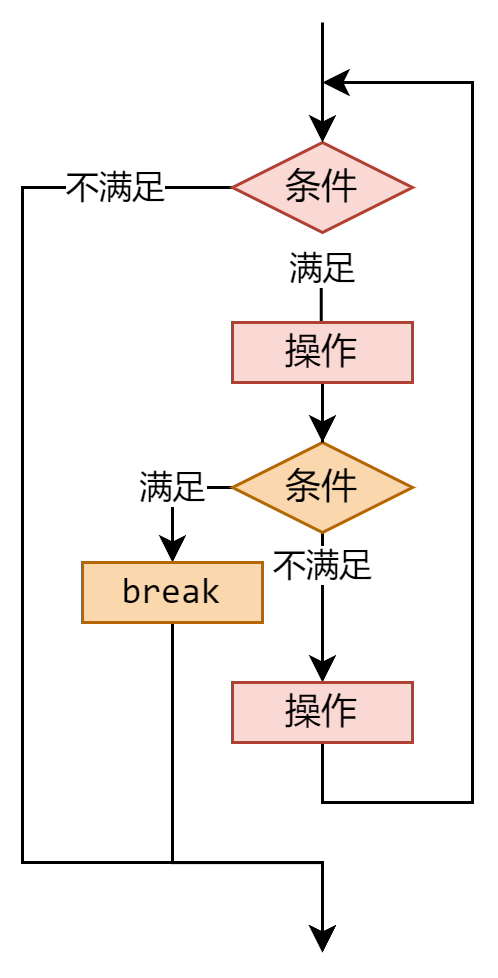
\includegraphics[width=0.35\textwidth]{../images/generalized_parts/03_structure_of_break.png}
    \caption{\lstinline@break@ 结构的流程图}
\end{figure}
举例来说,我们可以用这种方式来重写代码3.3的主函数部分,效果相同。
\begin{lstlisting}
    int num; //定义num,可不初始化
    while (true) { //永远循环,靠内部的break可以退出循环
        cin >> num; //输入num
        if (!cin) { //如果cin状态不正常,将执行break语句
            break; //退出该循环
        }
        if (num % 2 == 0) { //可以不用定义中间变量mod,直接用num%2来表示
            cout << "偶数" <<endl;
        }
        else {
            cout << "奇数" <<endl;
        }
    }
\end{lstlisting}
在这里,我们用 \lstinline@!cin@ 来作为判断条件,如果 \lstinline@cin@ 遭遇了不正常输入,它隐式转换会得到 \lstinline@false@,那么 \lstinline@!cin@ 就是 \lstinline@true@,于是 \lstinline@break@ 就会执行。\par
在 \lstinline@while@ 语句中,\lstinline@break@ 执行的效果是直接退出循环,后面的内容也不再执行。在 \lstinline@for@ 语句中,\lstinline@break@ 执行的效果也是直接退出循环,而且迭代操作也不会执行(因为即将退出循环,就没有迭代的必要了)。\par
读者需要特别注意:\textbf{\lstinline@break@ 语句只能退出当前所在的循环或 \lstinline@switch@-\lstinline@case@ 结构,而且只能退出一层。}我们不能使用 \lstinline@break@ 来退出 \lstinline@if@ 块(至少不能仅以退出 \lstinline@if@ 块为目的)。在上面的代码中我们也能看到,使用 \lstinline@break@ 的目的不是为了退出 \lstinline@if(!cin)@(虽然事实上也实现了这样的效果),而是为了退出 \lstinline@while(true)@。\par
请读者分析下面的代码,并猜测可能的输出结果,然后再自己运行一下,加以验证。
\begin{lstlisting}
    for (int i=0; i<5; i++) {
        for (int j=1; j<=5; j++) {
            if (i + j > 6) // 如果i+j>7就退出
                break; //会退出到哪里呢?
            cout << i * 5 + j << ' '; //每输出一个数字,以空格隔开
        }
        cout << endl; //换行
    }
\end{lstlisting}
实际的运行结果是\\\noindent\rule{\linewidth}{0.2pt}\texttt{
1 2 3 4 5\\
6 7 8 9 10\\
11 12 13 14\\
16 17 18\\
21 22
}\\\noindent\rule{\linewidth}{0.2pt}
从结果上可以看出,\lstinline@break@ 只退出了内层的 \lstinline@for@ 循环,而不会退出外层的 \lstinline@for@ 循环。否则它应该输出到 \lstinline@14@ 就彻底终止了。\par
再来看 \lstinline@continue@。它只能用于循环结构中,作用是跳过后面的代码,直接开始下一轮循环。\par
需要特别注意的是,\lstinline@continue@ 用在 \lstinline@for@ 循环中,不会跳过迭代操作。也就意味着,在 \lstinline@for@ 循环中使用 \lstinline@continue@ 不是``重新开始本轮循环'',而是``直接从下一轮循环开始''。\par
\begin{figure}[htbp]
   \centering
   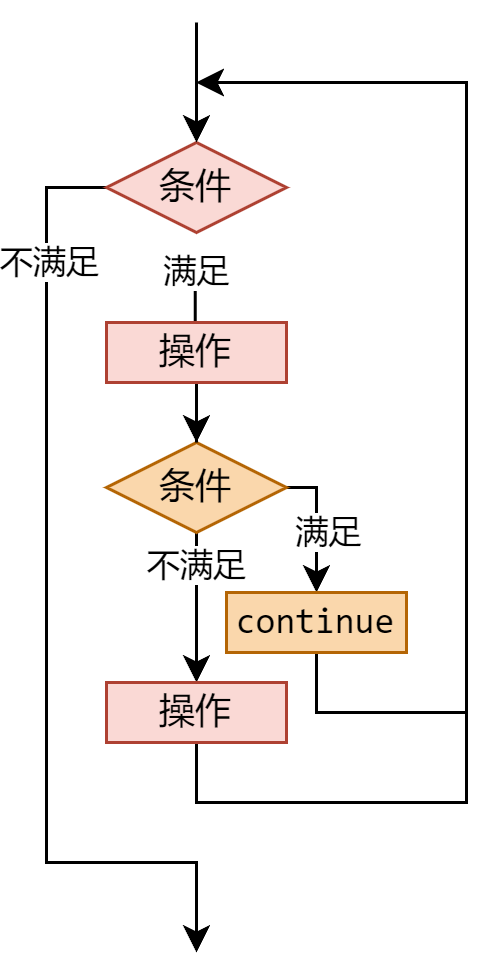
\includegraphics[width=0.35\textwidth]{../images/generalized_parts/03_structure_of_continue.png}
   \caption{\lstinline@continue@ 结构的流程图}
\end{figure}
\lstinline@continue@ 的用途很广泛,我们来举个实际一点的例子:有些时候,我们需要用户输入一些数字,但我们没有一个机制来防止用户输入不合理的内容(比如,需要用户输入数字,但用户却输入了字母)。一旦用户输入了不合理的内容,\lstinline@cin@ 就会进入错误状态,然后拒绝再读取输入。\par
为了让 \lstinline@cin@ 读取输入,我们需要清除状态,并清理输入流。我们暂时还不必关注这么多细节,我可以用一个简单的函数来把这项工作包揽:
\begin{lstlisting}
void input_clear() {
    cin.clear(); //清除错误状态
    while (cin.get() != '\n') //清除本行输入
        continue;
}
\end{lstlisting}
我们会在下一章讲函数,在此之前你只需要管怎么使用就可以了。\par
现在我们试着用这个方法来写一个输入数字求和的程序。用户可以输入若干整数,当输入 \lstinline@0@ 时结束循环,并给出以上所有数据的和。这里是完整代码:
\lstinputlisting[caption=\texttt{sum.cpp},label=lst:SumWithContinue]{../code_in_book/3.4/sum.cpp}
这段代码的主函数部分分别定义了 \lstinline@sum@ 和 \lstinline@x@,其中的 \lstinline@sum@ 用于求出所有数据的和,而 \lstinline@x@ 用于在每个迭代过程中存储新的数据。在 \lstinline@while@ 块内,程序将先读取 \lstinline@x@ 的输入。如果发现 \lstinline@cin@ 的状态不正常,就说明用户输入了不合理内容\footnote{实际情况可能更复杂,比如遇到了 \lstinline@EOF@。我们可以用一些代码来专门检测不正常的原因是否是 \lstinline@EOF@ 造成的,但是我们在本章还没必要细究这些问题。}。\par
如果用户读取了不合理内容,我们需要做两件事:一是将 \lstinline@cin@ 恢复到正常状态,以便下次输入;二是用 \lstinline@continue@ 跳过后面的部分,以防 \lstinline@sum+=x@ 误执行导致计算结果出现问题。\par
这里涉及到了一点复合赋值运算符的应用,我们简单一说便好:复合赋值运算符的返回值是赋值之后的左操作数的引用。比如加赋值,\lstinline@sum+=x@ 其实相当于 \lstinline@sum=sum+x@;减赋值,\lstinline@sum-=x@ 相当于 \lstinline@sum=sum-x@;还有乘赋值、除赋值、模赋值等运算符,它们都可以按照相同的规律来解释。\par
